\documentclass[12pt,letterpaper]{article}
\usepackage{graphicx,textcomp}
\usepackage{natbib}
\usepackage{setspace}
\usepackage{fullpage}
\usepackage{color}
\usepackage[reqno]{amsmath}
\usepackage{amsthm}
\usepackage{fancyvrb}
\usepackage{amssymb,enumerate}
\usepackage[all]{xy}
\usepackage{endnotes}
\usepackage{lscape}
\newtheorem{com}{Comment}
\usepackage{float}
\usepackage{hyperref}
\newtheorem{lem} {Lemma}
\newtheorem{prop}{Proposition}
\newtheorem{thm}{Theorem}
\newtheorem{defn}{Definition}
\newtheorem{cor}{Corollary}
\newtheorem{obs}{Observation}
\usepackage[compact]{titlesec}
\usepackage{dcolumn}
\usepackage{tikz}
\usetikzlibrary{arrows}
\usepackage{multirow}
\usepackage{xcolor}
\newcolumntype{.}{D{.}{.}{-1}}
\newcolumntype{d}[1]{D{.}{.}{#1}}
\definecolor{light-gray}{gray}{0.65}
\usepackage{url}
\usepackage{listings}
\usepackage{color}

\definecolor{codegreen}{rgb}{0,0.6,0}
\definecolor{codegray}{rgb}{0.5,0.5,0.5}
\definecolor{codepurple}{rgb}{0.58,0,0.82}
\definecolor{backcolour}{rgb}{0.95,0.95,0.92}

\lstdefinestyle{mystyle}{
	backgroundcolor=\color{backcolour},   
	commentstyle=\color{codegreen},
	keywordstyle=\color{magenta},
	numberstyle=\tiny\color{codegray},
	stringstyle=\color{codepurple},
	basicstyle=\footnotesize,
	breakatwhitespace=false,         
	breaklines=true,                 
	captionpos=b,                    
	keepspaces=true,                 
	numbers=left,                    
	numbersep=5pt,                  
	showspaces=false,                
	showstringspaces=false,
	showtabs=false,                  
	tabsize=2
}
\lstset{style=mystyle}
\newcommand{\Sref}[1]{Section~\ref{#1}}
\newtheorem{hyp}{Hypothesis}

\title{Problem Set 3
		Applied Stats/Quant Methods 1}
\date{Due: November 12, 2026}
\author{Samantha Richter}


\begin{document}
	\maketitle
	\section*{Instructions}
	\begin{itemize}
		\item Please show your work! You may lose points by simply writing in the answer. If the problem requires you to execute commands in \texttt{R}, please include the code you used to get your answers. Please also include the \texttt{.R} file that contains your code. If you are not sure if work needs to be shown for a particular problem, please ask.
	\item Your homework should be submitted electronically on GitHub.
	\item This problem set is due before 23:59 on Thursday November 12, 2026. No late assignments will be accepted.

	\end{itemize}

		\vspace{.25cm}
	
\noindent In this problem set, you will run several regressions and create an add variable plot (see the lecture slides) in \texttt{R} using the \texttt{incumbents\_subset.csv} dataset. Include all of your code.

	\vspace{.5cm}
\section*{Question 1}
\vspace{.25cm}
\noindent We are interested in knowing how the difference in campaign spending between incumbent and challenger affects the incumbent's vote share. 
	\begin{enumerate}
		\item Run a regression where the outcome variable is \texttt{voteshare} and the explanatory variable is \texttt{difflog}.		
		
		\noindent Before running the models, I looked at the dataset's structure and at the two variables used for this problem. \texttt{voteshare} is the incumbent's share of the vote, measured as a proportion between 0 and 1. \texttt{difflog} is the logged difference between the incumbent's and the challenger's campaign spending. Positive values indicate that the incumbent outspent the challenger, and negative values indicate the opposite.
		
		\lstinputlisting[language=R, firstline=36, lastline=52]{PS03.R}
		
		\begin{table} [H]
			\begin{center}
				\begin{tabular}{l c}
					\hline
					& Model 1 \\
					\hline
					(Intercept) & $0.579^{***}$ \\
					& $(0.002)$     \\
					difflog     & $0.042^{***}$ \\
					& $(0.001)$     \\
					\hline
					R$^2$       & $0.367$       \\
					Adj. R$^2$  & $0.367$       \\
					Num. obs.   & $3193$        \\
					\hline
					\multicolumn{2}{l}{\scriptsize{$^{***}p<0.001$; $^{**}p<0.01$; $^{*}p<0.05$}}
				\end{tabular}
				\caption{Regression of voteshare on difflog}
				\label{table:model1}
			\end{center}
		\end{table}
		
		\noindent The coefficient on \texttt{difflog} is positive (around 0.042) and statistically significant at the 0.001 level. So, there is a positive relationship between the logged spending difference and the incumbent's vote share. Since \texttt{voteshare} is a proportion, a one-unit increase in the logged difference in spending is associated with an average increase of about 0.042, or 4.2 percentage points, in the incumbent's vote share. 
		
		\noindent The intercept (0.579) means that when both candidates spend the same amount (\texttt{difflog} = 0), the model predicts that the incumbent will win about 57.9\% of the vote. The $R^2$ of 0.367 means that the logged spending difference between the incumbent and challenger explains about 36.7\% of the variation in incumbents' vote share. This is describing an observed association, so it's not necessarily a causal effect.
		\vspace{1cm}
		
		\item Make a scatterplot of the two variables and add the regression line. 	
		\lstinputlisting[language=R, firstline=54, lastline=63]{PS03.R}
		\begin{center}
			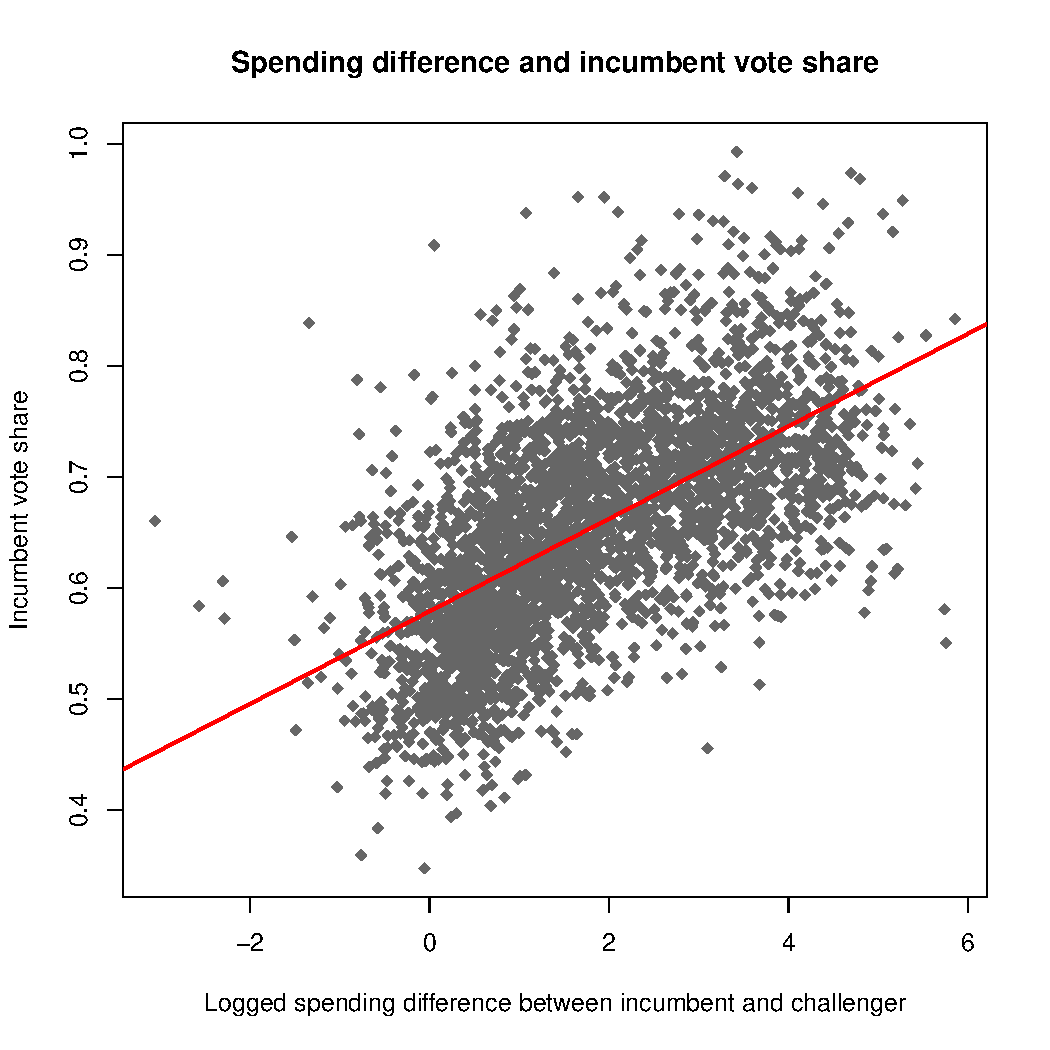
\includegraphics[width=.6\textwidth]{scatter1.pdf}
		\end{center}
		
		\noindent The plot shows that there is a positive relationship between the logged spending difference and the incumbent's vote share. As \texttt{difflog} increases, the points and the regression line move upwards. Most districts have a \texttt{difflog} between 0 and 4, so in most races the incumbent outspends the challenger. There are only a few districts on the left side of the plot where the challenger spent more. A large proportion of the vote shares are above 0.5, meaning the incumbents win in most districts regardless of spending, which makes sense with the intercept of 0.579.
		
		\noindent The vertical distance between each point and the line is that district's residual. The points are pretty spread out around the line, with incumbents at the same level of spending getting anywhere from about 50\% to 80\% of the vote. This makes sense with the moderate $R^2$. Spending helps to predict the vote share on average, but a lot of the variation comes from other factors. There are also a few outliers, such as districts where the incumbent spent much less than the challenger but still won significantly.
		\vspace{1cm}
		
		\item Save the residuals of the model in a separate object.
		\lstinputlisting[language=R, firstline=65, lastline=68]{PS03.R}
		\noindent The residuals are saved in \texttt{model1\_resid} to be used for question 4. Each residual is the observed vote share minus the vote share predicted by the model, so it is the part of \texttt{voteshare} that \texttt{difflog} does not explain.  
			\vspace{1cm}
			
		\item Write the prediction equation.
		\lstinputlisting[language=R, firstline=70, lastline=72]{PS03.R}
		\begin{verbatim}
			(Intercept)     difflog 
			0.579       0.042 
		\end{verbatim}
		
		\noindent The general bivariate prediction equation is written first, followed by the equation plugged in with the estimates from model 1. 
		\begin{align*}
			\hat{y} &= \hat{\beta}_0 + \hat{\beta}_1 \times x \\
			\widehat{\text{voteshare}} &= 0.579 + 0.042 \times \text{difflog}
		\end{align*}
		\noindent The model predicts that an incumbent who spends the same amount as their challenger will get approximately 57.9\% of the vote on average, and that their predicted vote share goes up by about 4.2 percentage points, on average, for every one-unit increase in \texttt{difflog}.
	\end{enumerate}
\newpage

\section*{Question 2}
\noindent We are interested in knowing how the difference between incumbent and challenger's spending and the vote share of the presidential candidate of the incumbent's party are related.	\vspace{.25cm}
	\begin{enumerate}
		\item Run a regression where the outcome variable is \texttt{presvote} and the explanatory variable is \texttt{difflog}.
		
		\noindent \texttt{presvote} is the vote share of the presidential candidate from the incumbent's party within each district. It is also measured as a proportion between 0 and 1. The predictor is the same as in Question 1, but now the outcome is the presidential vote instead of the incumbent's personal vote.
		\lstinputlisting[language=R, firstline=74, lastline=86]{PS03.R}
		
		\begin{table} [H]
			\begin{center}
				\begin{tabular}{l c}
					\hline
					& Model 2 \\
					\hline
					(Intercept) & $0.508^{***}$ \\
					& $(0.003)$     \\
					difflog     & $0.024^{***}$ \\
					& $(0.001)$     \\
					\hline
					R$^2$       & $0.088$       \\
					Adj. R$^2$  & $0.088$       \\
					Num. obs.   & $3193$        \\
					\hline
					\multicolumn{2}{l}{\scriptsize{$^{***}p<0.001$; $^{**}p<0.01$; $^{*}p<0.05$}}
				\end{tabular}
				\caption{Regression of presvote on difflog}
				\label{table:model2}
			\end{center}
		\end{table}
		
		\noindent The coefficient on \texttt{difflog} is positive (around 0.024) and statistically significant at the 0.001 level. So, districts where the incumbent outspends the challenger by more also tend to give a higher vote share to the presidential candidate of the incumbent's party. A one-unit increase in \texttt{difflog} is associated with an average increase of about 0.024, or 2.4 percentage points, in the presidential candidate's vote share.
		
		\noindent The intercept (0.508) means that when both candidates spend the same amount, the model predicts that the presidential candidate of the incumbent's party gets about 50.8\% of the vote share in that district. The $R^2$ is 0.088, meaning the logged spending difference explains about 8.8\% of the variation in presidential vote share. The relationship is statistically significant but not a strong one. Again, this is an association and not a causal effect. A potential explanation is that both variables are driven by how popular the party is in the district.
		\vspace{1cm}
		
		\item Make a scatterplot of the two variables and add the regression line. 
		\lstinputlisting[language=R, firstline=88, lastline=97]{PS03.R}
		\begin{center}
			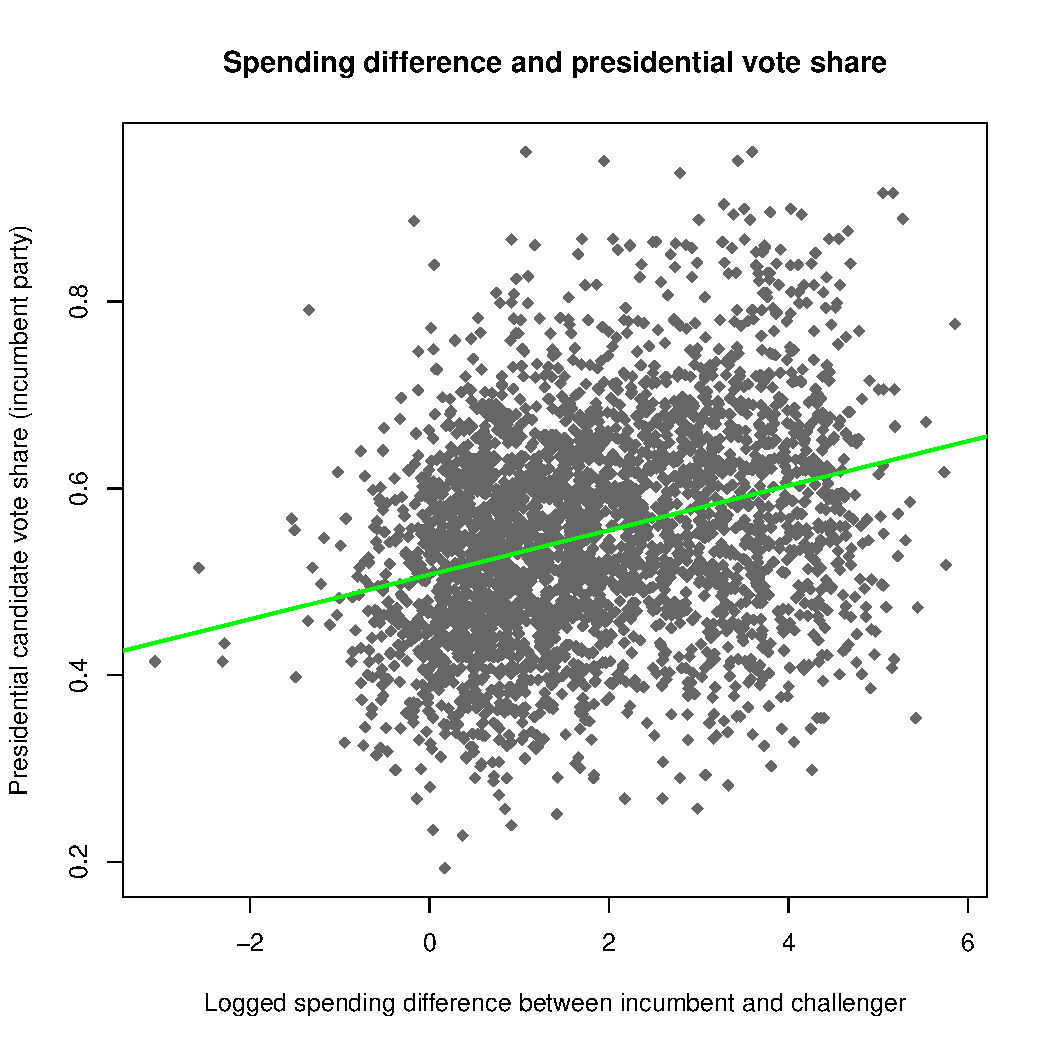
\includegraphics[width=.6\textwidth]{scatter2.pdf}
		\end{center}
		
		\noindent The plot shows a slight positive relationship, but the slope is flatter than in Question 1 and the points are much more spread out. Since the \texttt{difflog} values are the same as in Question 1, the points are spread the same way horizontally, with most districts between 0 and 4. The difference is on the vertical axis. The presidential vote share ranges from around 0.2 to above 0.9, and many districts fall below 0.5. This means that the presidential candidate of the incumbent's party often lost in districts where the incumbent was reelected.
		
		\noindent The presidential vote share varies widely at almost all levels of spending, so the points don't cluster tightly around the line. This makes sense given the low $R^2$ of 0.088. Knowing the logged spending difference tells us  little about how the presidential candidate did in a given district. Comparing this plot to Question 1 shows that spending is much more strongly related to the incumbent's own vote share than to the presidential vote.
		\vspace{1cm}
		
		\item Save the residuals of the model in a separate object.	
		\lstinputlisting[language=R, firstline=99, lastline=102]{PS03.R}
		\noindent I saved the residuals in \texttt{model2\_resid} for question 4. Each residual is the observed presidential vote share minus the share predicted by the model, so it is the part of \texttt{presvote} that \texttt{difflog} does not explain.
		\vspace{1cm}
		
		\item Write the prediction equation.
		\lstinputlisting[language=R, firstline=104, lastline=106]{PS03.R}
		\begin{verbatim}
			(Intercept)     difflog 
			0.508       0.024 
		\end{verbatim}
		
		\begin{align*}
			\widehat{\text{presvote}} &= 0.508 + 0.024 \times \text{difflog}
		\end{align*}
		\noindent The model predicts that when the incumbent and challenger spend the same amount, the presidential candidate of the incumbent's party will get approximately 50.8\% of the vote in that district on average, and that this goes up by about 2.4 percentage points, on average, for every one-unit increase in \texttt{difflog}.
	\end{enumerate}
	
	\newpage	
\section*{Question 3}

\noindent We are interested in knowing how the vote share of the presidential candidate of the incumbent's party is associated with the incumbent's electoral success.
	\vspace{.25cm}
	\begin{enumerate}
		\item Run a regression where the outcome variable is \texttt{voteshare} and the explanatory variable is \texttt{presvote}.
		
		\noindent The outcome is the incumbent's vote share again, same as in Question 1, but the predictor is now the presidential candidate's vote share (from Question 2) instead of the logged spending difference. Both variables are proportions between 0 and 1.
		
		\lstinputlisting[language=R, firstline=108, lastline=118]{PS03.R}
		
		\begin{table} [H]
			\begin{center}
				\begin{tabular}{l c}
					\hline
					& Model 3 \\
					\hline
					(Intercept) & $0.441^{***}$ \\
					& $(0.008)$     \\
					presvote    & $0.388^{***}$ \\
					& $(0.013)$     \\
					\hline
					R$^2$       & $0.206$       \\
					Adj. R$^2$  & $0.206$       \\
					Num. obs.   & $3193$        \\
					\hline
					\multicolumn{2}{l}{\scriptsize{$^{***}p<0.001$; $^{**}p<0.01$; $^{*}p<0.05$}}
				\end{tabular}
				\caption{Regression of voteshare on presvote}
				\label{table:model3}
			\end{center}
		\end{table}
		
		\noindent The coefficient on \texttt{presvote} is positive (around 0.388) and statistically significant at the 0.001 level. So, this shows that incumbents tend to do better in districts where the presidential candidate of their party also did well. Since both variables are proportions, a one-unit increase in \texttt{presvote} would mean going from 0\% to 100\% of the vote. It is easier to think about this interpretation in percentage points. That would mean a 1 percentage point increase in the presidential candidate's vote share is associated with an average increase of about 0.39 percentage points in the incumbent's vote share.
		
		\noindent The intercept of 0.441 is the predicted vote share for an incumbent in a district where the presidential candidate of their party got 0\% of the vote. No districts in the data are anywhere near this, so the intercept doesn't have a meaningful interpretation on its own. The $R^2$ of 0.206 means that presidential vote share explains about 20.6\% of the total variation in the incumbents' vote share. This is less than the logged spending difference explained in Question 1. Just as with the other models, this is an association and not a causal effect. The presidential vote and the incumbent's vote are both likely to reflect how popular the party is in the district, so it may not mean that one is directly causing the other.
		\vspace{1cm}
		
		\item Make a scatterplot of the two variables and add the regression line. 
		\lstinputlisting[language=R, firstline=120, lastline=129]{PS03.R}
		\begin{center}
			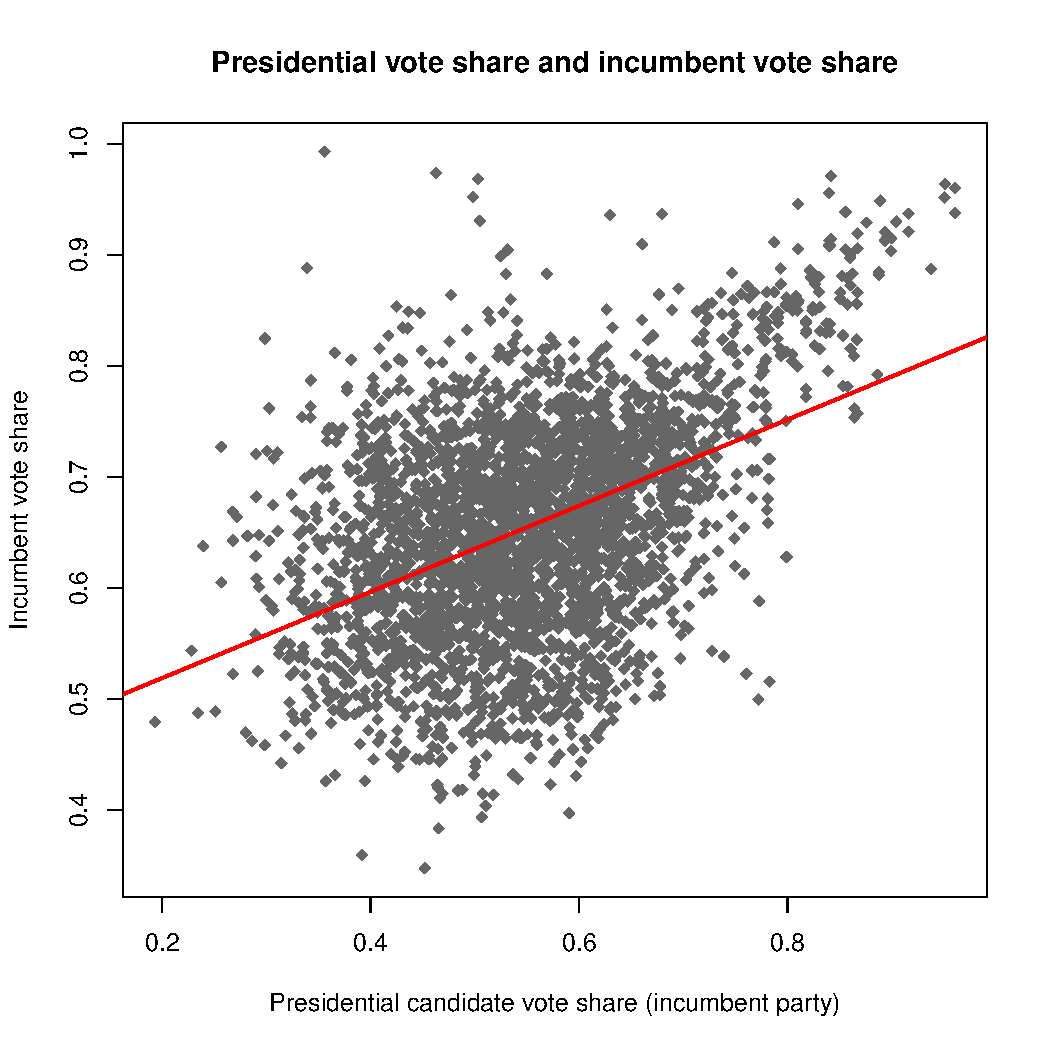
\includegraphics[width=.6\textwidth]{scatter3.pdf}
		\end{center}
		
		\noindent The plot shows that there is a positive relationship between the two vote shares. In places where the presidential candidate did better (districts further to the right), the incumbent vote shares tend to be higher. Most districts have a presidential vote share between about 0.4 and 0.7, and an incumbent vote share between about 0.5 and 0.8. There is a group of districts in the top right where both the presidential candidate and the incumbent did very well. These are likely districts where the party is very well liked.
		
		\noindent The scatterplot shows that incumbent vote shares are very frequently above 0.5, even in districts where the presidential candidate got less than half of the vote. This means incumbents often win in districts where their party's presidential candidate lost. This suggests that incumbents may have an advantage beyond just their party's popularity. The points are quite spread out around the line, which makes sense given the $R^2$ of 0.206. The presidential vote helps predict the incumbent's vote, but a lot of the variation is still unexplained.
		\vspace{1cm}
		
		\item Write the prediction equation.
		\lstinputlisting[language=R, firstline=131, lastline=133]{PS03.R}
		\begin{verbatim}
			(Intercept)    presvote 
			0.441       0.388 
		\end{verbatim}
		
		\begin{align*}
			\widehat{\text{voteshare}} &= 0.441 + 0.388 \times \text{presvote}
		\end{align*}
		
		\noindent The model predicts that in a district where the presidential candidate of the incumbent's party got 0\% of the vote, the incumbent would get approximately 44.1\% of the vote on average, although no districts in the data are close to this, so it's not meaningful in this context. The incumbent's predicted vote share goes up by approximately 0.39 percentage points, on average, for every 1 percentage point increase in \texttt{presvote}.
	\end{enumerate}
	

\newpage	
\section*{Question 4}
\noindent The residuals from part (a) tell us how much of the variation in \texttt{voteshare} is $not$ explained by the difference in spending between incumbent and challenger. The residuals in part (b) tell us how much of the variation in \texttt{presvote} is $not$ explained by the difference in spending between incumbent and challenger in the district.
	\begin{enumerate}
		\item Run a regression where the outcome variable is the residuals from Question 1 and the explanatory variable is the residuals from Question 2.	
		
		\noindent The outcome is \texttt{model1\_resid}, the part of the incumbent's vote share that is not explained by the logged spending difference. The predictor variable is \texttt{model2\_resid}, the part of the presidential vote share that is not explained by the logged spending difference. Since the influence of \texttt{difflog} has been removed from both variables, this regression shows how \texttt{presvote} and \texttt{voteshare} are related after accounting for spending. 
		
		\lstinputlisting[language=R, firstline=135, lastline=150]{PS03.R}
		
		\begin{table} [H]
			\begin{center}
				\begin{tabular}{l c}
					\hline
					& Model 4 \\
					\hline
					(Intercept)   & $-0.000$      \\
					& $(0.001)$     \\
					model2\_resid & $0.257^{***}$ \\
					& $(0.012)$     \\
					\hline
					R$^2$         & $0.130$       \\
					Adj. R$^2$    & $0.130$       \\
					Num. obs.     & $3193$        \\
					\hline
					\multicolumn{2}{l}{\scriptsize{$^{***}p<0.001$; $^{**}p<0.01$; $^{*}p<0.05$}}
				\end{tabular}
				\caption{Regression of Q1 residuals on Q2 residuals}
				\label{table:model4}
			\end{center}
		\end{table}
		
		\noindent The coefficient on \texttt{model2\_resid} is positive (about 0.257) and statistically significant at the 0.001 level. This means that in districts where the presidential candidate did better than the logged spending difference would predict (residual), the incumbent also tends to do better than the logged spending difference would predict. A one-unit increase in the Q2 residuals is associated with an average increase of approximately 0.257 in the Q1 residuals. This means that after accounting for the logged spending difference, a 1 percentage point increase in the presidential candidate's vote share is associated with an average increase of about 0.26 percentage points in the incumbent's vote share.
		
		\noindent This slope is smaller than the 0.388 from Question 3. In Question 3, part of the relationship between \texttt{presvote} and \texttt{voteshare} came from the fact that both are related to \texttt{difflog} (as shown in Questions 1 and 2). Once spending was accounted for in both variables, the remaining relationship is weaker, but still positive and significant.
		
		\noindent The intercept is essentially zero. This happens because residuals always average out to zero. The OLS line ensures that the points above it and below it balance out. Both variables in this model are residuals, so both have an average of zero. A regression line always passes through the average of $x$ and the average of $y$, so here it has to pass through (0, 0), which makes the intercept zero. The $R^2$ of about 0.130 means that the presidential vote explains about 13\% of the variation in incumbents' vote share that was unexplained by spending in Question 1.
	
		\vspace{1cm}
		\item Make a scatterplot of the two residuals and add the regression line. 
		\lstinputlisting[language=R, firstline=152, lastline=162]{PS03.R}
		\begin{center}
			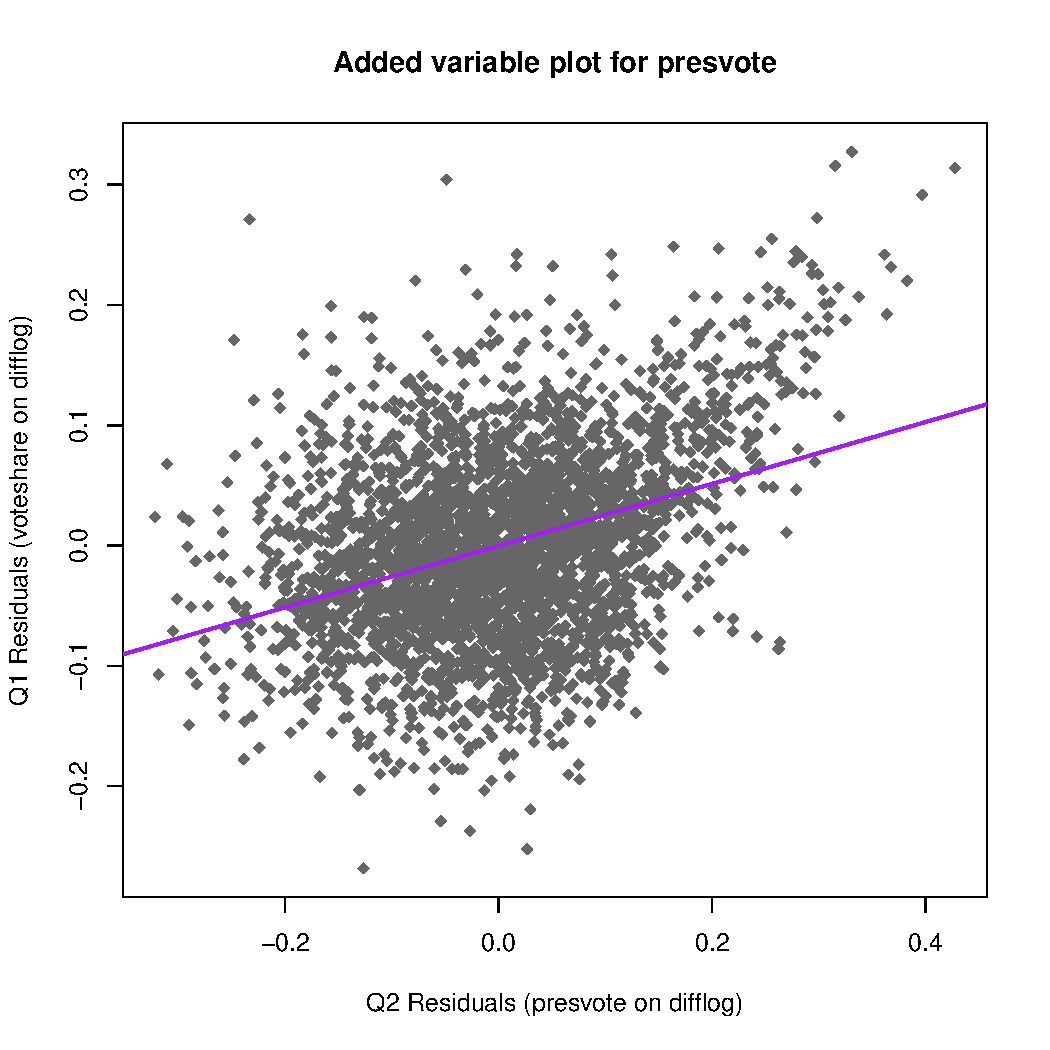
\includegraphics[width=.6\textwidth]{scatter4.pdf}
		\end{center}
		
		\noindent This scatterplot is an added variable plot. It shows the relationship between the variables \texttt{presvote} and \texttt{voteshare} after the influence of \texttt{difflog} has been removed from both. Unlike the previous scatterplots, both the x and y axes are centered around zero because residuals average to zero (explained above). Points on the right side are districts where the presidential candidate did better than the spending would predict, and points near the top are districts where the incumbent did better than the spending would predict.
		
		\noindent The regression line slopes upwards and passes through (0, 0), which shows the positive relationship that is left after accounting for spending. The points are in a loose, non tightly clustered, cloud around the line, which makes sense with the $R^2$ of 0.130. Even after removing spending, the presidential vote only explains a small part of what is left of the incumbent's vote share. Compared to the plot in Question 3, the line here is flatter since it has a smaller slope.
		\vspace{1cm}
		\item Write the prediction equation.
		
		\lstinputlisting[language=R, firstline=164, lastline=166]{PS03.R}
		\begin{verbatim}
			(Intercept) model2_resid 
			0.000        0.257 
		\end{verbatim}
		
		\begin{align*}
			\widehat{\text{model1\_resid}} &= 0 + 0.257 \times \text{model2\_resid}
		\end{align*}
		
		\noindent The model predicts that a district where the presidential vote is exactly what spending would predict (a Q2 residual of 0) will also have an incumbent vote share that is, on average, what spending would predict (a Q1 residual of 0). For every 1 percentage point that the presidential vote is above what spending predicts, the incumbent's vote share is approximately 0.26 percentage points above what spending predicts, on average.
		
	\end{enumerate}
	
	\newpage	

\section*{Question 5}
\noindent What if the incumbent's vote share is affected by both the president's popularity and the difference in spending between incumbent and challenger? 
	\begin{enumerate}
		\item Run a regression where the outcome variable is the incumbent's \texttt{voteshare} and the explanatory variables are \texttt{difflog} and \texttt{presvote}.	
		
		\noindent This is now a multiple regression with two predictors. Adding \texttt{presvote} with a \texttt{+} means each coefficient now shows the relationship between that variable and \texttt{voteshare} while holding the other variable constant.
		
		\lstinputlisting[language=R, firstline=169, lastline=179]{PS03.R}
		
	\begin{table} [H]
		\begin{center}
			\begin{tabular}{l c}
				\hline
				& Model 5 \\
				\hline
				(Intercept) & $0.449^{***}$ \\
				& $(0.006)$     \\
				difflog     & $0.036^{***}$ \\
				& $(0.001)$     \\
				presvote    & $0.257^{***}$ \\
				& $(0.012)$     \\
				\hline
				R$^2$       & $0.450$       \\
				Adj. R$^2$  & $0.449$       \\
				Num. obs.   & $3193$        \\
				\hline
				\multicolumn{2}{l}{\scriptsize{$^{***}p<0.001$; $^{**}p<0.01$; $^{*}p<0.05$}}
			\end{tabular}
			\caption{Regression of voteshare on difflog and presvote}
			\label{table:model5}
		\end{center}
	\end{table}
		
		\noindent Both coefficients are positive and statistically significant at the 0.001 level. The coefficient on \texttt{difflog} (around 0.036) means that, holding the presidential vote share constant, a one-unit increase in \texttt{difflog} is associated with an average increase of approximately 3.6 percentage points in the incumbent's vote share. The coefficient on \texttt{presvote} (around 0.257) means that, holding the logged spending difference constant, a 1 percentage point increase in the presidential candidate's vote share is associated with an average increase of approximately 0.26 percentage points in the incumbent's vote share.
		
		\noindent Both coefficients are smaller than in the bivariate models. The \texttt{difflog} coefficient went from 0.042 in Question 1 to 0.036 here, and the \texttt{presvote} coefficient went from 0.388 in Question 3 to 0.257 here. This is because \texttt{difflog} and \texttt{presvote} are related to each other (as Question 2 showed), so in the bivariate models each one was partly picking up the effect of the other. Once both are in the same model, each coefficient only shows the part of the relationship that belongs to that variable. The drop is much larger for \texttt{presvote}, which means a notable amount of its relationship with \texttt{voteshare} in Question 3 was connected to spending.
		
		\noindent The intercept (0.449) is the predicted vote share when both \texttt{difflog} and \texttt{presvote} are zero. Since no district has a presidential vote share near zero, the intercept doesn't have a meaningful interpretation on its own. The $R^2$ of 0.450 means the two variables together explain about 45\% of the variation in incumbents' vote share. This is higher than either variable explained alone, but lower than the two added together independently, because some of their explained variation overlaps. Again, these cannot be understood as causal effects.
		\vspace{1cm}
		
		\item Write the prediction equation.
		\lstinputlisting[language=R, firstline=181, lastline=183]{PS03.R}
		\begin{verbatim}
		(Intercept)     difflog    presvote 
		0.449       0.036       0.257
		\end{verbatim}
		
		\begin{align*}
			\widehat{\text{voteshare}} &= 0.449 + 0.036 \times \text{difflog} + 0.257 \times \text{presvote}
		\end{align*}
		
		\noindent The model predicts that for two districts with the same presidential vote, the incumbent's vote share goes up by about 3.6 percentage points on average for every one-unit increase in \texttt{difflog}. For two districts with the same logged spending difference, the incumbent's vote share goes up by about 0.26 percentage points on average for every 1 percentage point increase in the presidential vote. 
		\vspace{1cm}
		
		\item What is it in this output that is identical to the output in Question 4? Why do you think this is the case?
		\lstinputlisting[language=R, firstline=185, lastline=206]{PS03.R}
		\begin{verbatim}
		> c(se_model5, se_model4)
		[1] 0.012 0.012
		> se_model5 == se_model4
		[1] TRUE
		> all(res_model5 == res_model4)
		[1] TRUE
		> slope_model5
		presvote 
		0.256877 
		> slope_model4
		model2_resid 
		0.256877 
		> round(slope_model5, 6) == round(slope_model4, 6)
		presvote 
		TRUE 
		\end{verbatim}
		
		\noindent The estimated coefficient on \texttt{presvote} in this model (0.257) and its standard error (0.012) are the same as the coefficient and standard error on \texttt{model2\_resid} in Question 4. The checks in R confirm that the slopes, the standard errors, and the residuals all match. So, both models give the same estimate and the same uncertainty (se) around it.
		
		\noindent The intercept is 0.449 here but 0 in Question 4, because the Question 4 model uses residuals, which average to zero. Model 4 also doesn't have an estimated coefficient for \texttt{difflog}, since \texttt{difflog} was never included as a predictor there. Instead, its influence was removed from both variables beforehand.
		
		\noindent The coefficients are the same because both models are estimating the average partial effect of \texttt{presvote} on \texttt{voteshare}. The average partial effect is the average change in the incumbent's vote share associated with the presidential vote share, after taking into account how the logged spending difference influences the variation in vote share. The multiple regression in Question 5 does this in one step by including \texttt{difflog} in the model itself. Question 4 does it in steps, by first removing the part of both \texttt{voteshare} and \texttt{presvote} explained by \texttt{difflog} (Questions 1 and 2), and then regressing what is left of one on the other. Both approaches isolate the same part of the relationship, so they produce the same coefficient and standard error.
		\end{enumerate}




\end{document}
